\documentclass{article}


\usepackage{arxiv}

\usepackage[utf8]{inputenc} % allow utf-8 input
\usepackage[T1]{fontenc}    % use 8-bit T1 fonts
\usepackage{hyperref}       % hyperlinks
\usepackage{url}            % simple URL typesetting
\usepackage{booktabs}       % professional-quality tables
\usepackage{amsfonts}       % blackboard math symbols
\usepackage{nicefrac}       % compact symbols for 1/2, etc.
\usepackage{microtype}      % microtypography
\usepackage{lipsum}
\usepackage{listings}
\usepackage{color}
\usepackage{graphicx}

\definecolor{dkgreen}{rgb}{0,0.6,0}
\definecolor{gray}{rgb}{0.5,0.5,0.5}
\definecolor{mauve}{rgb}{0.58,0,0.82}
\setcounter{page}{8}
\title{Ray Tracing and Animation, accelerated with OpenACC}


\lstset{frame=tb,
  language=PHP,
  aboveskip=3mm,
  belowskip=3mm,
  showstringspaces=false,
  columns=flexible,
  basicstyle={\small\ttfamily},
  numbers=none,
  numberstyle=\tiny\color{gray},
  keywordstyle=\color{blue},
  commentstyle=\color{dkgreen},
  stringstyle=\color{mauve},
  breaklines=true,
  breakatwhitespace=true,
  tabsize=3
}


\author{
  Quinn Vinlove\\%\thanks{Use footnote for providing further
    %information about author (webpage, alternative
    %address)---\emph{not} for acknowledging funding agencies.} \\
  Mathematics \& Computer Science Major\\
  Lewis \& Clark College\\
  Portland, OR 97219 \\
  \texttt{quinnvinlove@lclark.edu} \\
  %% examples of more authors
   %\And
 %Elias D.~Striatum \\
  %Department of Electrical Engineering\\
  %Mount-Sheikh University\\
  %Santa Narimana, Levand \\
  %\texttt{stariate@ee.mount-sheikh.edu} \\
  %% \AND
  %% Coauthor \\
  %% Affiliation \\
  %% Address \\a
  %% \texttt{email} \\
  %% \And
  %% Coauthor \\
  %% Affiliation \\
  %% Address \\
  %% \texttt{email} \\
  %% \And
  %% Coauthor \\
  %% Affiliation \\
  %% Address \\
  %% \texttt{email} \\
}

\begin{document}
\maketitle

\begin{abstract}
Ray tracing is a method used to render complex scenes in non-time intensive situations. Generating animation frames with ray tracing multiplies the computational complexity of it. Through the use of OpenACC pragmas in a program that implemented both ray tracing and animation in C, I was able to see a 30\% speed increase, without having to write GPU Native code. While this approach was not as effective as traditional methods of graphics programming, it allowed for a gentle, introduction to GPU programming that isn’t bound to any particular GPU vendor, while offering potential for future investigation through MPI.
\end{abstract}


% keywords can be removed
\keywords{Computer Graphics \and OpenACC \and Parallel Programming 
}


\section{Introduction}
Offline rendering is a term used to describe all rendering that doesn’t need to happen in real time, and thus can be used for more complex shapes and animations. Animation itself is a good use case for High-Performance computing because it involves rendering many frames, increasing the computational complexity of the problem significantly. 


\section{Materials}
\label{sec:headings}
I chose to use the OpenACC parallel programming model to render animations, because it provided a more welcoming introduction into the world of GPU programming, allowing for the use of ‘regular’ C and C++ syntax that is accelerated with pragmas. 
All code was compiled with PGI Compiler v. 19.4. Non-Accelerated code was compiled with the -fast flag. For this project, I used interactive gpu-small sessions inside of the Pittsburgh Supercomputing Center BRIDGES supercomputer, using a NVIDIA Tesla-P100 graphics card.


\section{Methods}
I wrote a simple ray tracer in C, then added on the ability to move objects with a control loop. My end goal was to show the orbit of the earth around the sun, and the moon around the earth, because ray tracers are particularly good at rendering spheres. Input was read from a custom scene file and output into a series of 256-color bitmap files. 
	My first target for optimizing the code I wrote was to unroll the two nested for loops and place them in a kernel. Because the ray tracer casts a ray for every pixel of the output file, running that process in a massively parallel environment across many GPU cores would result in speedup. But, there were some difficulties associated with that. Every subroutine called within the loop needed an acc routine seq pragma before it. I also relied heavily on global variables, which aren’t always explicitly copied in or out inside of kernel regions. Ultimately, I rewrote my code to remove globals, which reduced the amount of data copied to the GPU. Perhaps the largest issue, however, was the size of the output array. I used a 2d array of structs to hold pixel color information, and my target array size, 1920x1080 pixels (equivalent to 1080p resolution), meant that I had to declare that variable on the heap instead of the stack. OpenACC struggled to move such a large amount of data into the GPU (Fig. 1), and it wasn’t until I reduced the array size to 854x480 pixels (equivalent to 480p) and placed the variable on the stack did OpenACC return a satisfactory result. I rendered 365 frames at this resolution, to simulate the 365 days in an earth year. (Fig. 2)

\section{Results}
Without OpenACC, my code rendered the animation in 38.999s, as measured by the Linux time utility. With the OpenACC flag enabled, the animation was rendered in 29.989s. The use of OpenACC with this particular code sample resulted in a 1.3x speedup. (Fig. 3)

\section{Discussion}

The small performance increase offered by OpenACC could have been caused by memory transfer speed and management issues. Even the ‘reduced size’ output array has to be copied out of the GPU with every new frame rendered. And the memory management issue I ran into which resulted in the unique output graphic could be alleviated by breaking the output frame into different ‘slices,’ allowing for higher-resolution output. 
A GPU Native language, like CUDA, is probably a better choice for Computer Graphics problems, due to it’s built-in vector types and other features which make it ideal. But the universal nature of OpenACC allows it to compile to any platform, making development easier and not bound to one particular hardware or software vendor. 
	Additionally, because only one frame could be rendered at a time, this application could benefit from MPI, and sending each frame to a thread with it’s own GPU, effectively creating a hybrid MPI/OpenACC job. 

\section{Conclusion}

Overall, the speedup I saw was encouraging, and OpenACC could prove to be a useful tool for introductory computer graphics classes or other situations where ease of use and understanding of the underlying GPU model takes priority over raw speed. 

\begin{figure}
    \centering
    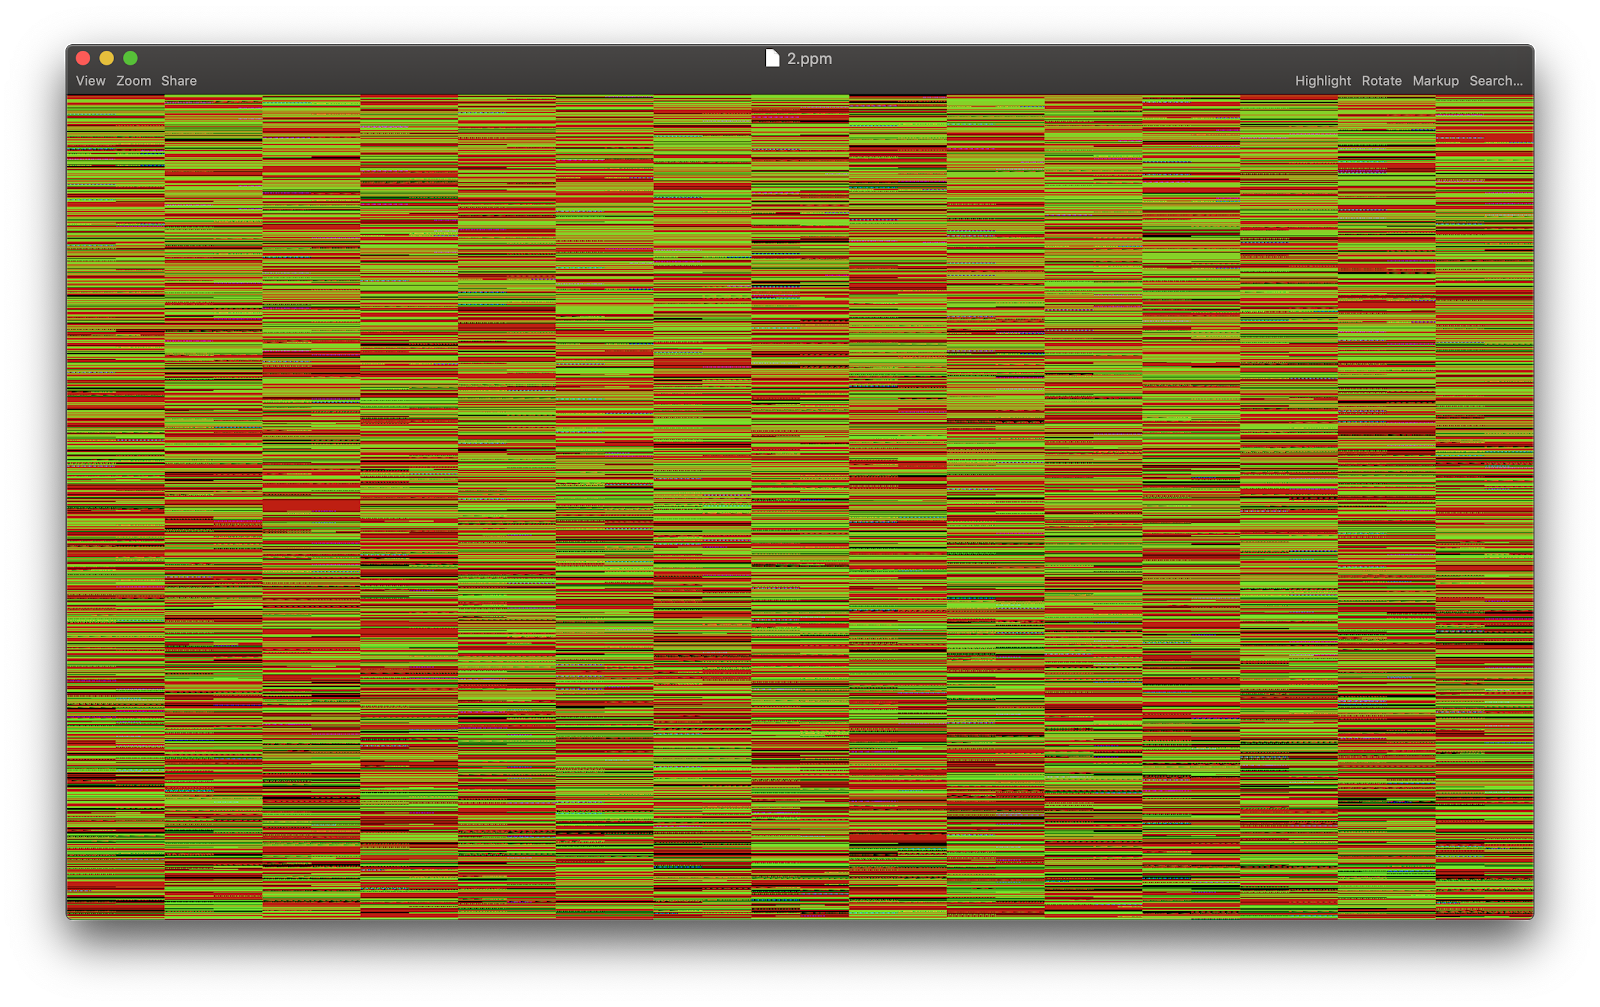
\includegraphics[width=.9\columnwidth]{quinn_fig1.png}
    \caption{GPU Glitch}
    \label{fig:my_label}
\end{figure}

\begin{figure}
    \centering
    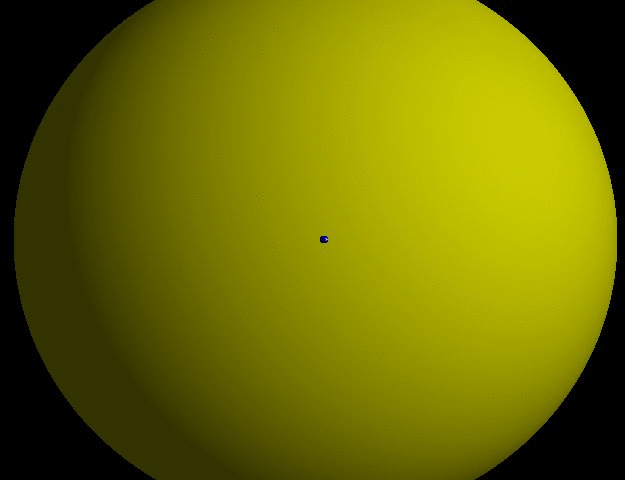
\includegraphics[width=.9\columnwidth]{quinn_fig2.png}
    \caption{Final Product}
    \label{fig:my_label}
\end{figure}

\section{Runtimes}
\begin{verbatim}


With OpenACC:
real	0m29.989s
user	0m25.733s
sys	0m1.314s

Without OpenACC:
real	0m38.999s
user	0m34.634s
sys	0m1.281s
\end{verbatim}


%\bibliographystyle{unsrt}  
%\bibliography{references}  %%% Remove comment to use the external .bib file (using bibtex).
%%% and comment out the ``thebibliography'' section.


%%% Comment out this section when you \bibliography{references} is enabled.
%\begin{thebibliography}{1}

%\bibitem{aaa}
%Chapple, M.
%\newblock Creating Databases and Tables in SQL
%\newblock In {\em Life Wire, 2019}

%\end{thebibliography}

\section{Link to Code}
Code is at \href{https://github.com/quin2/rayaccel}{https://github.com/quin2/rayaccel}
\end{document}
